%Version 3 October 2023
% See section 11 of the User Manual for version history
%
%%%%%%%%%%%%%%%%%%%%%%%%%%%%%%%%%%%%%%%%%%%%%%%%%%%%%%%%%%%%%%%%%%%%%%
%%                                                                 %%
%% Please do not use \input{...} to include other tex files.       %%
%% Submit your LaTeX manuscript as one .tex document.              %%
%%                                                                 %%
%% All additional figures and files should be attached             %%
%% separately and not embedded in the \TeX\ document itself.       %%
%%                                                                 %%
%%%%%%%%%%%%%%%%%%%%%%%%%%%%%%%%%%%%%%%%%%%%%%%%%%%%%%%%%%%%%%%%%%%%%

%%\documentclass[referee,sn-basic]{sn-jnl}% referee option is meant for double line spacing

%%=======================================================%%
%% to print line numbers in the margin use lineno option %%
%%=======================================================%%

%%\documentclass[lineno,sn-basic]{sn-jnl}% Basic Springer Nature Reference Style/Chemistry Reference Style

%%======================================================%%
%% to compile with pdflatex/xelatex use pdflatex option %%
%%======================================================%%

%%\documentclass[pdflatex,sn-basic]{sn-jnl}% Basic Springer Nature Reference Style/Chemistry Reference Style


%%Note: the following reference styles support Namedate and Numbered referencing. By default the style follows the most common style. To switch between the options you can add or remove �Numbered� in the optional parenthesis. 
%%The option is available for: sn-basic.bst, sn-vancouver.bst, sn-chicago.bst%  
 
%\documentclass[sn-nature]{sn-jnl}% Style for submissions to Nature Portfolio journals
%\documentclass[referee, lineno, pdflatex, sn-basic]{sn-jnl}% Basic Springer Nature Reference Style/Chemistry Reference Style
\documentclass[referee, lineno, sn-mathphys-num]{sn-jnl}% Math and Physical Sciences Numbered Reference Style 
%%\documentclass[sn-mathphys-ay]{sn-jnl}% Math and Physical Sciences Author Year Reference Style
%%\documentclass[sn-aps]{sn-jnl}% American Physical Society (APS) Reference Style
%%\documentclass[sn-vancouver,Numbered]{sn-jnl}% Vancouver Reference Style
%%\documentclass[sn-apa]{sn-jnl}% APA Reference Style 
%%\documentclass[sn-chicago]{sn-jnl}% Chicago-based Humanities Reference Style

%%%% Standard Packages
%%<additional latex packages if required can be included here>

\usepackage{graphicx}%
\usepackage{multirow}%
\usepackage{amsmath,amssymb,amsfonts}%
\usepackage{amsthm}%
\usepackage{mathrsfs}%
\usepackage[title]{appendix}%
\usepackage{xcolor}%
\usepackage{textcomp}%
\usepackage{manyfoot}%
\usepackage{booktabs}%
\usepackage{algorithm}%
\usepackage{algorithmicx}%
\usepackage{algpseudocode}%
\usepackage{listings}%
%%%%

%%%%%=============================================================================%%%%
%%%%  Remarks: This template is provided to aid authors with the preparation
%%%%  of original research articles intended for submission to journals published 
%%%%  by Springer Nature. The guidance has been prepared in partnership with 
%%%%  production teams to conform to Springer Nature technical requirements. 
%%%%  Editorial and presentation requirements differ among journal portfolios and 
%%%%  research disciplines. You may find sections in this template are irrelevant 
%%%%  to your work and are empowered to omit any such section if allowed by the 
%%%%  journal you intend to submit to. The submission guidelines and policies 
%%%%  of the journal take precedence. A detailed User Manual is available in the 
%%%%  template package for technical guidance.
%%%%%=============================================================================%%%%

%% as per the requirement new theorem styles can be included as shown below
\theoremstyle{thmstyleone}%
\newtheorem{theorem}{Theorem}%  meant for continuous numbers
%%\newtheorem{theorem}{Theorem}[section]% meant for sectionwise numbers
%% optional argument [theorem] produces theorem numbering sequence instead of independent numbers for Proposition
\newtheorem{proposition}[theorem]{Proposition}% 
%%\newtheorem{proposition}{Proposition}% to get separate numbers for theorem and proposition etc.

\theoremstyle{thmstyletwo}%
\newtheorem{example}{Example}%
\newtheorem{remark}{Remark}%

\theoremstyle{thmstylethree}%
\newtheorem{definition}{Definition}%

\raggedbottom
%%\unnumbered% uncomment this for unnumbered level heads

\begin{document}

\title[Coin-Switching Strategy for High-Frequency Trading in Cryptocurrencies Using an Actor-Critic Model and Trend Disentanglement]{Coin-Switching Strategy for High-Frequency Trading in Cryptocurrencies Using an Actor-Critic Model and Trend Disentanglement}

%%=============================================================%%
%% GivenName	-> \fnm{Joergen W.}
%% Particle	-> \spfx{van der} -> surname prefix
%% FamilyName	-> \sur{Ploeg}
%% Suffix	-> \sfx{IV}
%% \author*[1,2]{\fnm{Joergen W.} \spfx{van der} \sur{Ploeg} 
%%  \sfx{IV}}\email{iauthor@gmail.com}
%%=============================================================%%

\author[1]{\fnm{Ahmad} \sur{Asadi}}\email{ahmad.asadi@aut.ac.ir}

\author*[1]{\fnm{Reza} \sur{Safabakhsh}}\email{safa@aut.ac.ir}
%\equalcont{These authors contributed equally to this work.}

\affil*[1]{\orgdiv{Computer Engineering Department}, \orgname{Amirkabir University of Technology}, \orgaddress{\street{Hafez St.}, \city{Tehran}, \postcode{1591634311}, \state{Tehran}, \country{Iran}}}


%%==================================%%
%% Sample for unstructured abstract %%
%%==================================%%

\abstract{This paper presents a novel framework for cryptocurrency portfolio management, focusing on high-frequency trading (HFT) scenarios, where decisions are made based on predicting near-future trend changes in the asset prices. The framework leverages a Variational Autoencoder (VAE) to disentangle the price behavior of cryptocurrencies into trends and variances, enabling the prediction of trend shifts. A deep reinforcement learning (DRL) model is used to dynamically switch investments between assets, focusing on the single cryptocurrency with the most promising trend at each hour. This coin-switching strategy, in contrast to traditional diversification models, reduces risk while optimizing returns by reallocating investments based on real-time trend predictions. Experimental results demonstrate that the proposed model significantly outperforms state-of-the-art strategies in terms of total returns, achieving a remarkable total return on investment of over 1850\%, while reducing maximum drawdowns to just -13.3\%. These findings highlight the effectiveness of the dynamic coin-switching strategy in maximizing returns and mitigating risks in highly volatile cryptocurrency markets.}

%%================================%%
%% Sample for structured abstract %%
%%================================%%

% \abstract{\textbf{Purpose:} The abstract serves both as a general introduction to the topic and as a brief, non-technical summary of the main results and their implications. The abstract must not include subheadings (unless expressly permitted in the journal's Instructions to Authors), equations or citations. As a guide the abstract should not exceed 200 words. Most journals do not set a hard limit however authors are advised to check the author instructions for the journal they are submitting to.
% 
% \textbf{Methods:} The abstract serves both as a general introduction to the topic and as a brief, non-technical summary of the main results and their implications. The abstract must not include subheadings (unless expressly permitted in the journal's Instructions to Authors), equations or citations. As a guide the abstract should not exceed 200 words. Most journals do not set a hard limit however authors are advised to check the author instructions for the journal they are submitting to.
% 
% \textbf{Results:} The abstract serves both as a general introduction to the topic and as a brief, non-technical summary of the main results and their implications. The abstract must not include subheadings (unless expressly permitted in the journal's Instructions to Authors), equations or citations. As a guide the abstract should not exceed 200 words. Most journals do not set a hard limit however authors are advised to check the author instructions for the journal they are submitting to.
% 
% \textbf{Conclusion:} The abstract serves both as a general introduction to the topic and as a brief, non-technical summary of the main results and their implications. The abstract must not include subheadings (unless expressly permitted in the journal's Instructions to Authors), equations or citations. As a guide the abstract should not exceed 200 words. Most journals do not set a hard limit however authors are advised to check the author instructions for the journal they are submitting to.}

\keywords{disentangled representation learning, high frequency trading, deep reinforcement learning, stock portfolio management, variational auto-encoders}

%%\pacs[JEL Classification]{D8, H51}

%%\pacs[MSC Classification]{35A01, 65L10, 65L12, 65L20, 65L70}

\maketitle


\section{Introduction}
High-frequency trading (HFT) models have revolutionized financial markets, becoming a cornerstone of modern stock and cryptocurrency trading. While traditional HFT focuses on capitalizing on millisecond-level market inefficiencies, a growing body of research highlights the importance of developing models that operate on longer, but still high-resolution, time frames such as hourly intervals. In volatile markets like cryptocurrencies, hourly price movements capture significant trends and reversals, providing opportunities for strategic portfolio adjustments. By leveraging advanced algorithms, real-time analysis, and frequent decision-making, models operating at this granularity can effectively identify short-term price patterns, optimize asset allocation, and enhance portfolio performance. The success of such strategies lies in their ability to respond quickly to evolving market conditions, maximizing returns while mitigating risk over frequent but manageable trading intervals.

A critical aspect of HFT strategies is the prevention of small, cumulative losses, which can have an outsized impact on long-term portfolio performance. Unlike traditional trading, where losses can be balanced over extended periods, HFT operates on razor-thin margins and high transaction volumes, making small losses particularly detrimental. When left unchecked, these losses can compound rapidly, eroding gains and leading to substantial underperformance. Conversely, mitigating minor losses through precise data-driven decision-making can result in exponential returns over time. This dynamic underscores the importance of developing models capable of analyzing micro-level price behaviors and reacting swiftly to unfavorable conditions.

High-frequency trading techniques rely heavily on integrating diverse information sources to identify and capitalize on market trends. Advanced models aggregate technical indicators \cite{chen2018profitability}, quantitative financial data \cite{gomber2015high}, crowd-sourced sentiment analysis \cite{liu2023multi}, and multi-source data fusion approaches \cite{asadi4423354multi, liu2023multi}. By combining these inputs, HFT models achieve a comprehensive understanding of the market behavior, improving their precision in trend detection and risk mitigation \cite{li2014online}. This multi-faceted approach empowers traders to not only avoid minor losses, but also uncover critical pivot points in stock price series key moments where trends shift direction. Identifying these pivot points before they occur is central to developing robust strategies capable of maximizing returns while navigating the market's inherent volatility and uncertainty.

While existing research emphasizes the importance of fusing data from multiple sources to identify price series pivot points, we argue that a deeper understanding of price behavior is necessary for predicting trend changes. The ability to anticipate these shifts requires disentangling the factors influencing price movements, such as trend direction and volatility, to predict the probability of changes in the trend of each asset's price in the near future. In highly dynamic markets like cryptocurrencies, even short-term price reversals can significantly impact trading strategies, making it essential to accurately forecast these changes to optimize portfolio performance.

A key innovation of this study is the introduction of a coin-switching strategy that challenges the conventional diversification approach typically employed in portfolio management. Diversification, which involves allocating investments across multiple assets \cite{markovitz1959portfolio}, is widely used to mitigate risk by reducing dependence on any single asset's performance. However, in high-frequency trading (HFT), where decisions are made at fine-grained time intervals, this traditional approach may not fully exploit opportunities arising from short-term price movements.

In the proposed model, the entire investment value is allocated to a single coin at the start of each investment period, based on the predicted probability of trend shifts for all available coins. This focused strategy enables the model to dynamically select the coin most likely to exhibit a favorable trend, effectively reducing risk while maximizing returns. By disentangling trends and variances for each coin, the model ensures that the selection is data-driven and reflective of the near-term market conditions. Over multiple investment periods, this coin-switching strategy behaves similarly to the cumulative effects of diversification, as the portfolio iteratively adapts to the market's most promising opportunities. Moreover, this approach parallels the concept of concurrent task execution in CPU processing, where tasks are executed in rapid succession to achieve results comparable to parallel computing.

In this paper, we propose a new framework for stock portfolio management that focuses on predicting the probability of near-future trend changes for each asset. The contributions of this study are as follows:

\begin{enumerate}
	\item We introduce a model that disentangles price behavior into meaningful components to predict the likelihood of trend shifts in each asset's price.
	\item We propose a deep reinforcement learning (DRL) model capable of dynamically switching between assets based on the predicted probabilities of trend changes.
	\item We propose a coin-switching strategy for high-frequency trading, where the entire investment is allocated to a single asset during each period. This approach, informed by disentangled trend and variance features, reduces risk while optimizing returns by focusing on the most promising asset at each interval.
	\item The proposed coin-switching method mirrors the cumulative effects of diversification over time by dynamically reallocating investments across assets, akin to concurrent task execution in CPUs.
	\item We demonstrate that the proposed model outperforms state-of-the-art portfolio management strategies in the cryptocurrency market, achieving superior returns and improved portfolio stability.
\end{enumerate}

By leveraging disentangled price features, reinforcement learning, and innovative allocation strategies, the proposed framework addresses the challenges of frequent decision-making in dynamic financial markets and enhances the ability to adapt to near-term price trends.

The rest of this paper is organized as follows: In Section 2 we review the existing models for stock portfolio management and stock price trend predictors. Section 3 describes in detail the structures of the time-series uncertainty estimation model and the deep reinforcement learning model. The proposed model is then evaluated and the results are reported and discussed in Section 4. Finally, the conclusions of the paper are summarized in Section 5.


\section{Related Work}

Reinforcement learning (RL) techniques, particularly deep reinforcement learning (DRL) provide excellent methods useful in portfolio management. DRL models are able to learn optimal trading policies through interactions with the market, adjusting asset allocations based on real-time data and the evolving market environment. These models can dynamically adjust portfolio weights by considering a wide range of factors, including price trends, volatility, and market sentiment. However, despite their potential, DRL models that rely on diversification may not be well-suited to handle the challenges posed by high-frequency trading in volatile markets like cryptocurrencies, where small fluctuations can quickly lead to losses.


Deep learning models have become an essential tool in stock portfolio management due to their ability to process vast amounts of data and identify complex patterns that traditional models often miss. Traditional portfolio management approaches typically rely on statistical models \cite{li2012pamr} or optimization techniques \cite{pennanen2012introduction} to guide investment decisions. With the rise of deep learning and deep reinforcement learning (DRL) methods, more sophisticated, data-driven strategies have emerged, often incorporating technical indicators for better portfolio management \cite{ayala2021technical,agrawal2022stock,taghian2021reinforcement,taghian2022learning}.

In financial markets, the ability of deep learning models to handle complex, multi-modal data has led to the adoption of information fusion techniques to improve portfolio management. One approach involves integrating multiple types of data, such as historical prices, financial statements, and social media sentiment, into a unified model, allowing for a more comprehensive market analysis \cite{asadi4423354multi}. Additionally, ensemble methods, which combine outputs from multiple models trained on different data subsets or architectures, have shown to enhance prediction accuracy and robustness \cite{carta2021multi}. Other advancements include the use of attention mechanisms to focus on relevant information across markets \cite{zhao2022stock} and the application of transformer models for fusing temporal data, which helps in optimizing portfolio performance by minimizing small losses \cite{gullotto2021portfolio,kisiel2022portfolio}. Finally, recent work by \citet{abdulsahib2024cross} introduces disentangled representation learning to capture shared features between markets, providing a more nuanced understanding of the market interdependencies and improving prediction accuracy.

The use of deep reinforcement learning (DRL) models in high-frequency trading (HFT) is expanding rapidly. \citet{asare2024deep} introduced a CNN-based model designed for generating 15-minute buy/sell signals for cryptocurrencies. \citet{sun2022deepscalper} developed DeepScalper, a model for intraday trading that combines a dueling Q-network to handle large action spaces and an encoder-decoder framework to extract multi-resolution temporal data. \citet{qin2024earnhft} proposed the EarnHFT model, a hierarchical RL framework that calculates optimal action-values using dynamic programming as a Q-teacher, creates a pool of diverse RL agents for different market trends, and employs a minute-level router to select an RL agent from the pool. \citet{zong2024macrohft} introduced MacroHFT, another hierarchical RL model that trains a router to choose agents from the pool, incorporating a memory-augmented, context-aware RL model to address agent biases. \citet{fatemi2024finvision} proposed a multi-modal, multi-agent system where specialized LLM-based agents process diverse financial data, such as news reports, candlestick charts, and trading signals.

Another approach in high-frequency trading involves predicting future prices and selecting portfolios based on these predictions. Despite challenges like high volatility and non-stationary data, deep learning and feature selection techniques show promise in cryptocurrency forecasting \cite{otabek2024prediction}. \citet{akyildirim2021prediction} explore the predictability of twelve cryptocurrencies using SVM-based machine learning models, achieving the best and most consistent results. \citet{ye2021predicting} uses ANNs to predict price directions for Bitcoin, Ethereum, and Cardano, effectively capturing complex patterns. \citet{liu2021forecasting} employ stacked denoising autoencoders for Bitcoin price prediction, managing both direction and level predictions. \citet{jay2020stochastic} integrate stochastic processes with neural networks to improve prediction accuracy.

While much of the related work has concentrated on integrating information from various sources for stock portfolio management, our study takes a different approach by focusing on the fundamental factors that drive price behavior. The objective is to identify early signs of trend shifts and anticipate price pivot points before they materialize. To achieve this, we introduce a model that disentangles price behavior into meaningful components, predicting the likelihood of trend changes for each asset. We propose an Actor-Critic model that dynamically switches between assets based on the predicted probabilities of trend changes, optimizing returns while managing risks. Additionally, we present a coin-switching strategy tailored for high-frequency trading, where investments are concentrated in a single asset during each period. This strategy, informed by disentangled trend and variance features, aims to reduce risk and maximize returns by focusing on the most promising asset. Furthermore, the coin-switching method effectively mirrors the cumulative benefits of diversification over time by reallocating investments across assets.





\section{Proposed Method}
The model proposed in this paper consists of two modules. The first module is a feature extractor which is enabled to extract features indicating the strength of the current price trend in the near future. The second module is an actor-critic based model which selects a single coin to buy and hold until the next investment interval based on the uncertainty about the price trends of each coin extracted by the first module. 

Figure \ref{fig:arch} illustrates the architecture of the model presented in this study. The model is built based on the concept of disentangled representation learning, where a feature extractor is trained to extract features from the historical price data of each coin. These extracted features are then combined and fed into an actor-critic model to select a single coin from the available options in the market. It is important to note that the portfolio proposals in this research consist of only one coin, and no combination of coins is considered. This constraint is imposed to enhance the clarity of the model's investigation and facilitate comparisons with the existing models in the field.


%In the context of stock trading, we approach the complex task by decomposing it into two distinct components: leveraging pre-trained deep learning models for portfolio management as expert models, and introducing a novel Model Switching Agent (MS Agent) designed to dynamically select the most suitable expert model based on the current state of the environment and the performance of each expert model. This two-pronged approach aims to enhance the adaptability and effectiveness of the overall trading system by intelligently switching between expert models to optimize decision-making in response to changing market conditions. Figure \ref{fig:arch} illustrates the structure of this idea.

\begin{figure}[H]
	\centering
	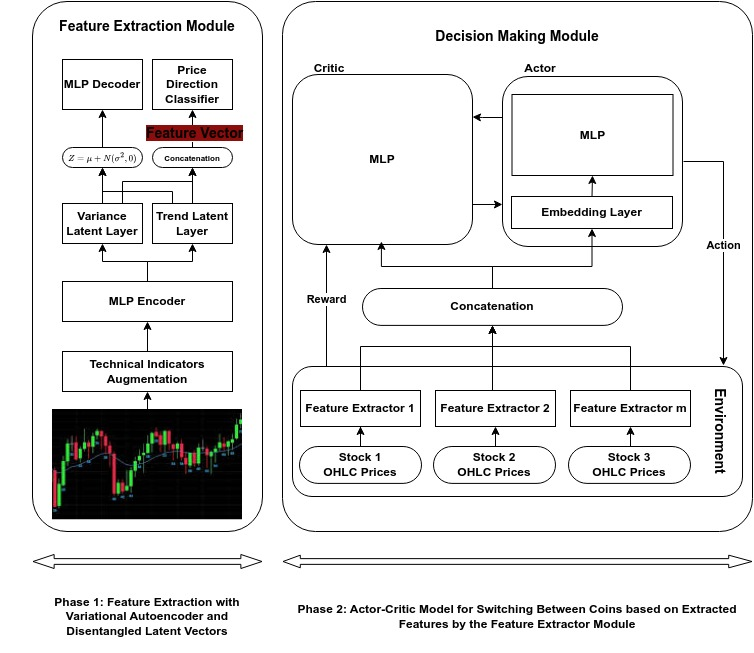
\includegraphics[scale=0.6]{./NewArch.jpg}
	\caption{Structure of the Model Switching approach for stock trading}
	\label{fig:arch}
\end{figure}


\subsection{Feature Extraction}

Disentangled representation learning is a powerful technique in machine learning that aims to learn representations of data where different factors of variation are separated into distinct and interpretable components. This can be particularly useful in time series data, where multiple underlying processes may be present and need to be disentangled for better understanding and analysis.

Let's consider a time series dataset $X = \{x^1, x^2, ..., x^t\}$, where $x^i$ represents the observation at time step $i$. The goal of disentangled representation learning on time series is to learn a set of latent variables $Z = \{z_1, z_2, ..., z_K\}$ that capture the underlying factors of variation in the data. These latent variables should be disentangled, meaning that each $z_k$ represents a different aspect of the data that is independent of the others.

Given the assumption of independence among the generating factors, the task of disentangled representation learning in a dimension-wise manner aims to encode the information pertaining to these generating factors by means of a latent vector of lower dimensionality - as a compact representation of the high-dimensional observations. The relationship between the observations and the latent vectors can be formally characterized by their joint distribution

\begin{align}
p_\theta(x,z) &= p_\theta(x|z) p_\theta(z) \label{eq:1}\\
p_\theta(z) &= N(z|0, \sigma^2 I) \label{eq:2}
\end{align}
where $\theta$ denotes the set of parameters of the feature extractor model and the prior distribution $p(z)$ is typically assumed to be a multidimensional Gaussian distribution with the same variance in all directions 


One common approach to achieve disentangled representation learning on time series data is through Variational Autoencoders (VAEs) \cite{duan2019unsupervised,li2022towards,li2021learning}. VAEs are generative models that learn a probabilistic mapping between the observed data and the latent variables. By introducing a prior distribution over the latent variables, VAEs can learn disentangled representations by encouraging the latent variables to capture independent factors of variation in the data.

In the first module of the proposed method, we utilize a VAE structure to capture the underlying distribution of the data and extract disentangled representations for uncertainty measurement in stock portfolio management. The VAE is designed to learn a latent space that separates different factors of variation in the data, enabling us to better understand and quantify the uncertainty associated with our model's predictions.

The VAE consists of an encoder network that maps input data (e.g., historical stock prices, market indicators) to a latent space representation, and a decoder network that reconstructs the input data from the latent space. By training the VAE to minimize the reconstruction error and maximize the mutual information between the input and latent representations, we aim to learn a compact and meaningful representation of the data that facilitates uncertainty estimation.

To encourage disentangled representation learning in the VAE, we incorporate regularization techniques, such as $\beta$-VAE \cite{burgess2018understanding} or disentanglement loss functions, that promote the separation of different factors of variation (e.g., market trends, individual stock performance) in the latent space. This disentangled representation enables us to measure uncertainty more effectively and make informed decisions in stock portfolio management.

The relation between the latent features and input data in the proposed VAE model is described in equation \eqref{eq:beta-vae}.

\begin{equation}
z_i = \hat{\mu_i} + \hat{\sigma_i} \epsilon
\label{eq:beta-vae}
\end{equation}

where $z_i$ denotes the $i$th element of the latent vector, $\hat{\mu_i}$ and $\hat{\sigma_i}$ respectively represent the latent vectors learned by the encoder to simulate the mean and variance of the price series, and $\epsilon \propto N(0, 1)$ denotes a random white noise.

Since the latent vectors $\hat{\mu_i}$ and $\hat{\sigma_i}$ are the vectors that are passed to the portfolio manager module, they are assumed to encode information regarding price trend. In addition, these vectors should be informative enough to estimate our uncertainty about the persistence of the current price trend in the near future. Therefore, a classifier is embedded inside the VAE model and an extra term is added to VAE model's loss function to ensure that $\hat{\mu_i}$ and $\hat{\sigma_i}$ encode necessary information.

A binary classifier $\Phi(\hat{\mu}, \hat{\sigma})$ is augmented into the VAE model in order to enforce latent variables to encode information related to the future price trend. The ground-truth labels for this classifier are generated via equation \eqref{eq:class1}.
\begin{equation}
Y_i^t = 
\begin{cases}
\text{1} &\quad\text{if } \dfrac{x_i^{t+l}}{x_i^t} > 1\\
\text{-1} &\quad\text{otherwise}
\end{cases}
\label{eq:class1}
\end{equation}
where $\dfrac{x_i^{t+l}}{x_i^t}$ computes the total return of stock $i$ in $l$ steps ahead from time step $t$ and $Y_i^t$ denotes the label of the classifier for stock $i$ in time step $t$. Based on equation \eqref{eq:class1}, the proposed loss function for learning the set of parameters of the VAE model is presented in equation \eqref{eq:lossVAE}.
\begin{align}
\mathcal{L} &= \mathcal{E}  + \mathcal{C} - \mathcal{K}	\label{eq:lossVAE}  \\
\mathcal{E} &= \Sigma_{i=1}^S \Sigma_{t=w}^T (\hat{X_i^t} - X_i^T) ^ 2 	\label{eq:lossVAE2} \\
\mathcal{C} &= \Sigma_{i=1}^S \Sigma_{t=w}^T \Gamma(\Phi(\hat{\mu_i^t}, \hat{\sigma_i^t}), Y_i^t) 	\label{eq:lossVAE3} \\
\mathcal{K} &= \frac{1}{2} \Sigma_{i=1}^S \Sigma_{t=w}^T (1 + log(\hat{\sigma_i^t})^2 - \hat{\mu_i^t}^2 - (\hat{\sigma_i^t})^2 	\label{eq:lossVAE1} 
\end{align}
where the loss function $\mathcal{L}$ for the VAE model is decomposed into three distinct components: $\mathcal{E}$ for reconstruction loss, $\mathcal{K}$ for Kullback-Leibler divergence, and $\mathcal{C}$ for the classification loss. Moreover, the variables $w$, $S$ and $T$ represent the window size, the number of stocks in the dataset, and the maximum time-step in the training set, respectively.

The VAE model undergoes training separately from the other components of the proposed model. The dataset necessary for training the VAE model comprises time-series data of stock historical prices divided into windows of size $w$, with the corresponding labels based on equation \eqref{eq:class1}.

\subsubsection{Stock Switching}

In the second part of our method, we propose an Actor-Critic neural network architecture for generating optimal stock portfolios over a set of liquid coins in the cryptocurrencies market. The Actor network learns a policy that selects one of the available stocks based on the current state of the market and the uncertainty estimates on current price trend of each stock provided by the VAE. The Critic network evaluates the value of the chosen actions and provides feedback to update the policy.

The Actor-Critic architecture leverages reinforcement learning techniques to optimize the stock portfolio management strategy over time, taking into account both the immediate rewards (e.g., profit/loss) and the long-term objectives (e.g., investment risk and returns in long run). By incorporating uncertainty measurements from the VAE into the decision-making process, our model can adapt to changing market conditions and make more robust portfolio recommendations.

Overall, our method combines disentangled representation learning with deep reinforcement learning to enhance stock portfolio management by effectively measuring uncertainty and optimizing portfolio decisions in the volatile cryptocurrencies market. Through this integrated approach, we aim to improve the performance, stability, and interpretability of AI-driven investment strategies for financial applications.

The Actor network is designed to generate actions based on the input data. It consists of two fully connected layers with LeakyReLU activation functions to introduce non-linearity and facilitate learning complex patterns. The final layer of the Actor network is a Softmax layer, which normalizes the output values into a probability distribution over the available actions. This distribution determines the action to be taken at each time step.

The Critic network is responsible for evaluating the actions generated by the Actor network. It consists of two fully connected layers, similar to the Actor network. However, the last layer of the Critic network contains only one node, which outputs a scalar value representing the estimated return associated with the generated action. The Critic network utilizes a logarithmic estimate of the return values as its reward function, providing a measure of the quality of the actions taken by the Actor network.

The overall structure of the Actor-Critic model is illustrated in Figure \ref{fig:arch}. The Actor network generates actions based on the input data, while the Critic network evaluates these actions to provide feedback to the Actor network. This feedback loop enables the model to learn and improve its trading strategies over time.


In addition, a novel immediate reward function is proposed. It calculates the difference between the immediate return of the model's proposed action and the optimal return achievable based on future prices of each coin. This reward function is defined in Equation \eqref{eq:ri}.
\begin{equation}
\mathcal{R}_t = log(\frac{1}{1 + [\Sigma_{j} a_j^t * R_j^t] - max_j(R_j^t)})
\label{eq:ri}
\end{equation}
where $\mathcal{R}_t$ denotes the immediate reward of the stock switching agent at time step $t$, $R^t = \{r_1^t, \cdots, r_n^t\}$ is the set of stock returns in which $r_i^t = \frac{X_i^{t+1}}{X_i^t}$ represents the next time-step return of stock $i$, and the $j$th element of the action vector at time step $t$ is denoted by $a_j^t$. The best immediate stock return is calculated as $max_j(R_j^t)$ and the return of the agent's action is computed as $ [\Sigma_{j} a_j^t * R_j^t]$. If the agent selects the best stock at time-step $t$, the difference between the action return and the best stock return is zero; otherwise, it is a negative value greater than $-1$. Equation \eqref{eq:ri} suggests that the maximum reward is attained when there is no difference between the agent's selection and the best stock.





\section{Experimental Results}
%\lipsum[2]

\subsection{The Dataset}

In our study, we analyze a dataset consisting of historical hourly OHLC (Open, High, Low, Close) data for the eight most liquid crypto exchanges in the market over the recent years. The exchanges chosen for our research are listed in Table \ref{tbl:data}.

\begin{table}[h]
	\centering
	\caption{List of selected exchanges in experimental data-set}
	\begin{tabular}{c|c|c|c}
		Symbol & Distinct Timestamp Count & First Timestamp & Last Timestamp \\
		\hline
		\hline
		ADA/BTC & 25982 & 2022-01-01& 2024-12-18 \\
		BNB/BTC & 25983 & 2022-01-01& 2024-12-18 \\
		BTC/USDT & 25981 & 2022-01-01& 2024-12-18 \\
		DASH/BTC & 25983 & 2022-01-01& 2024-12-18 \\
		EOS/BTC & 25982 & 2022-01-01& 2024-12-18 \\
		ETH/BTC & 25982 & 2022-01-01& 2024-12-18 \\
		LTC/BTC & 25980 & 2022-01-01& 2024-12-18 \\
		XRP/BTC & 25983 & 2022-01-01& 2024-12-18 \\
		
	\end{tabular}
	\label{tbl:data}
	
\end{table}

Figure \ref{fig:dataset} illustrates the hourly OHLC price histories for the exchanges in the dataset. This dataset provides a comprehensive view of the price movements and trends in the cryptocurrencies market, enabling us to evaluate the performance of the proposed method for stock portfolio management under real-world conditions. 

\begin{figure}[H]
	\centering
	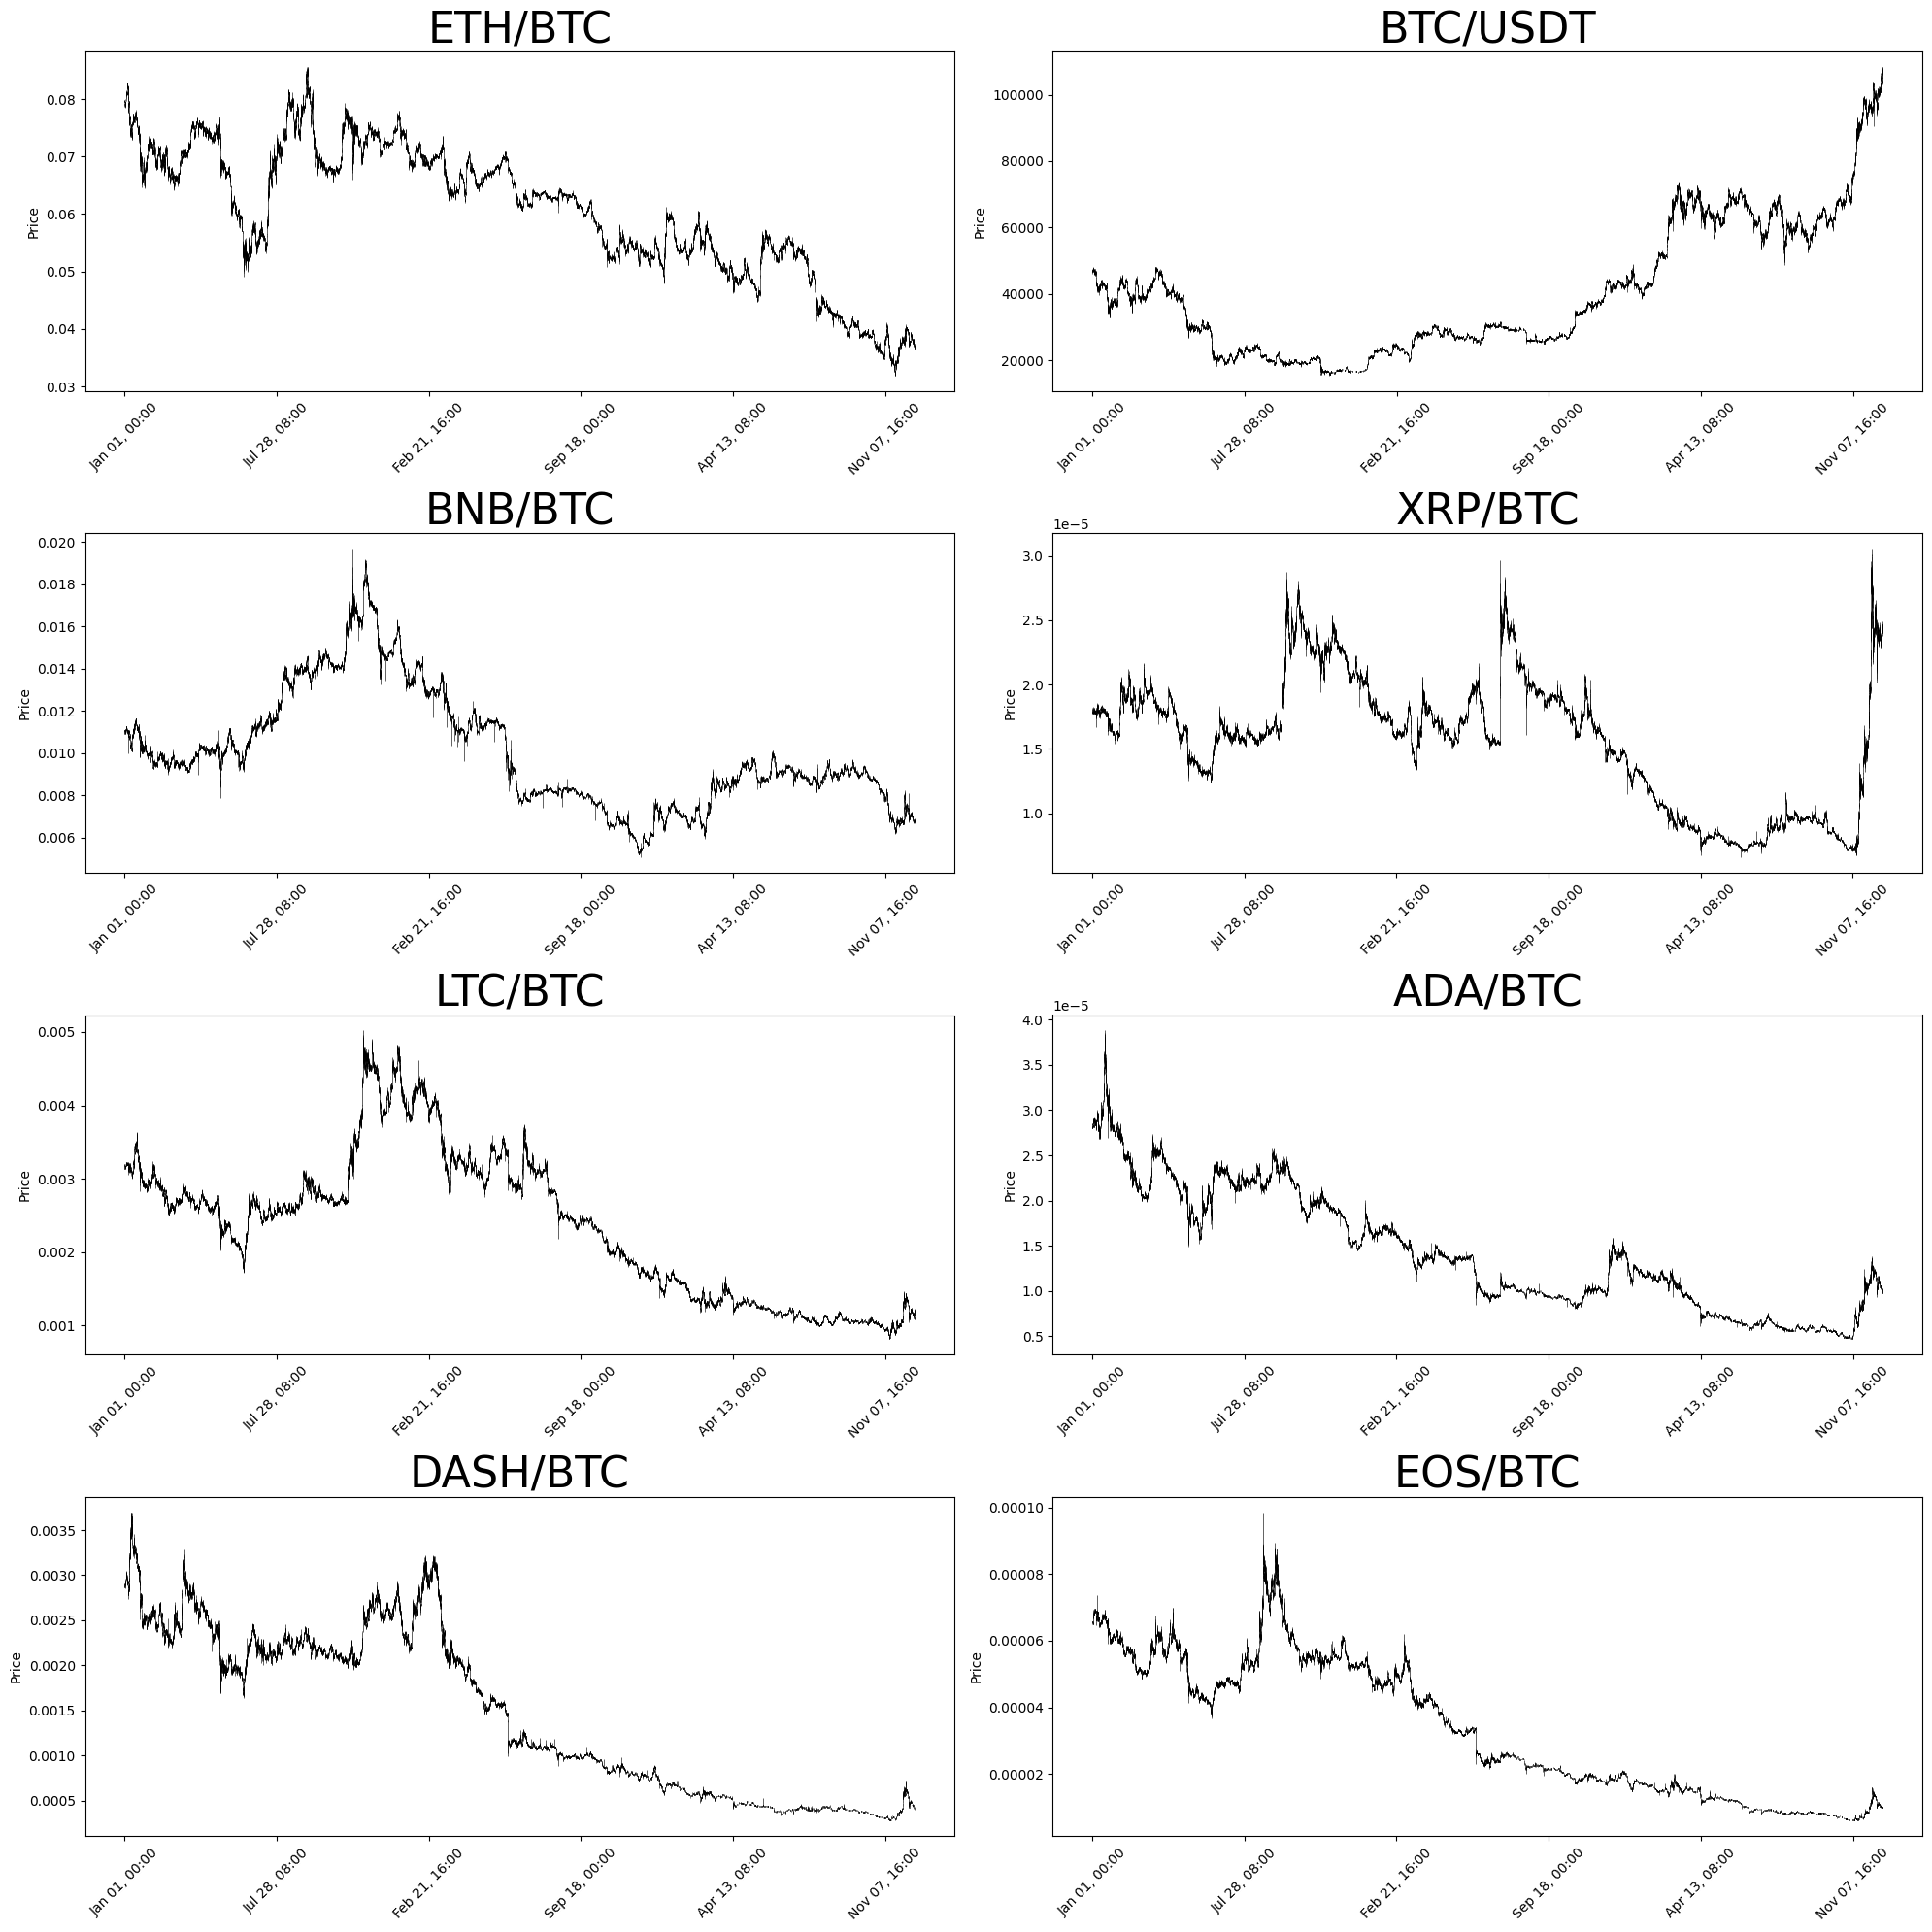
\includegraphics[scale=0.3]{./dataset.png}
	\caption{Illustration of the price series gathered in the dataset.}
	\label{fig:dataset}
\end{figure}



In the rest of this section we will investigate different aspects of the proposed model in portfolio management. Section 4.2 studies the features of the latent space learned by the VAE model. Section 4.3 provides an ablation study on the proposed model and a makes a comparison between the different versions of the proposed model. Section 4.4 compares the results of the proposed model with the baseline models.

\subsection{Latent Space Investigation}
In this experiment, we explored the latent space of a Variational Autoencoder (VAE) trained on time-series data. The model was designed to disentangle the input space into two distinct latent representations: one capturing the trend of the price series and the other representing the variance. To facilitate a focused analysis, the dimensionality of both the trend and variance variables was constrained to one. This simplification allowed for a straightforward visualization and interpretation of the latent space.

The encoder of the VAE outputs two latent variables, denoted as $\mu$ (mean) and $\sigma^2$ (variance), corresponding to the trend and variance representations. By iterating over the $\mu$-$\sigma^2$ space, we sampled time-series data using the decoder. These generated series were visualized in a 2D graph, where each point in the $\mu$-$\sigma^2$ grid corresponds to a generated time-series. The resulting graph contains 64 generated images arranged systematically across the latent space, divided into four distinct sub-spaces for analysis.

Figure \ref{fig:latent_full} demonstrates a 2D visualization as a comprehensive view of the latent space and its impact on the generated time-series. The graph is structured into four sub-spaces, with notable differences in the nature of the generated series:

\begin{enumerate}
	\item Upper sub-spaces:
	The generated series in the upper half of the latent space resembles the mathematical function $sin(x)$ for the range $-\frac{\pi}{2} < x < \frac{\pi}{2}$. These series exhibit smooth oscillations and a consistent periodicity, suggesting that the upper latent sub-spaces predominantly capture sinusoidal positive price trend.
	
	\item Lower sub-spaces:
	In the lower half of the latent space, the generated series align more closely with $sin(x)$ for the range $0 < x < \frac{\pi}{2}$. These series exhibit similar periodic behavior but with a phase shift compared to the upper sub-spaces, indicating a separation in phase dynamics within the latent representation.
	
\end{enumerate}

The primary contribution of this illustration is showcasing the VAE's ability to decompose price series into small wave-like patterns resembling sinusoidal functions in various phases. This indicates the model's capability to detect trend shifts effectively. By inputting a test time-series at each timestep, the VAE maps the historical price data into its trained latent space. The latent space then associates the input series with specific sub-spaces defined by the corresponding $\mu$ and $\sigma^2$ values.

\begin{figure}[h]
	\centering
	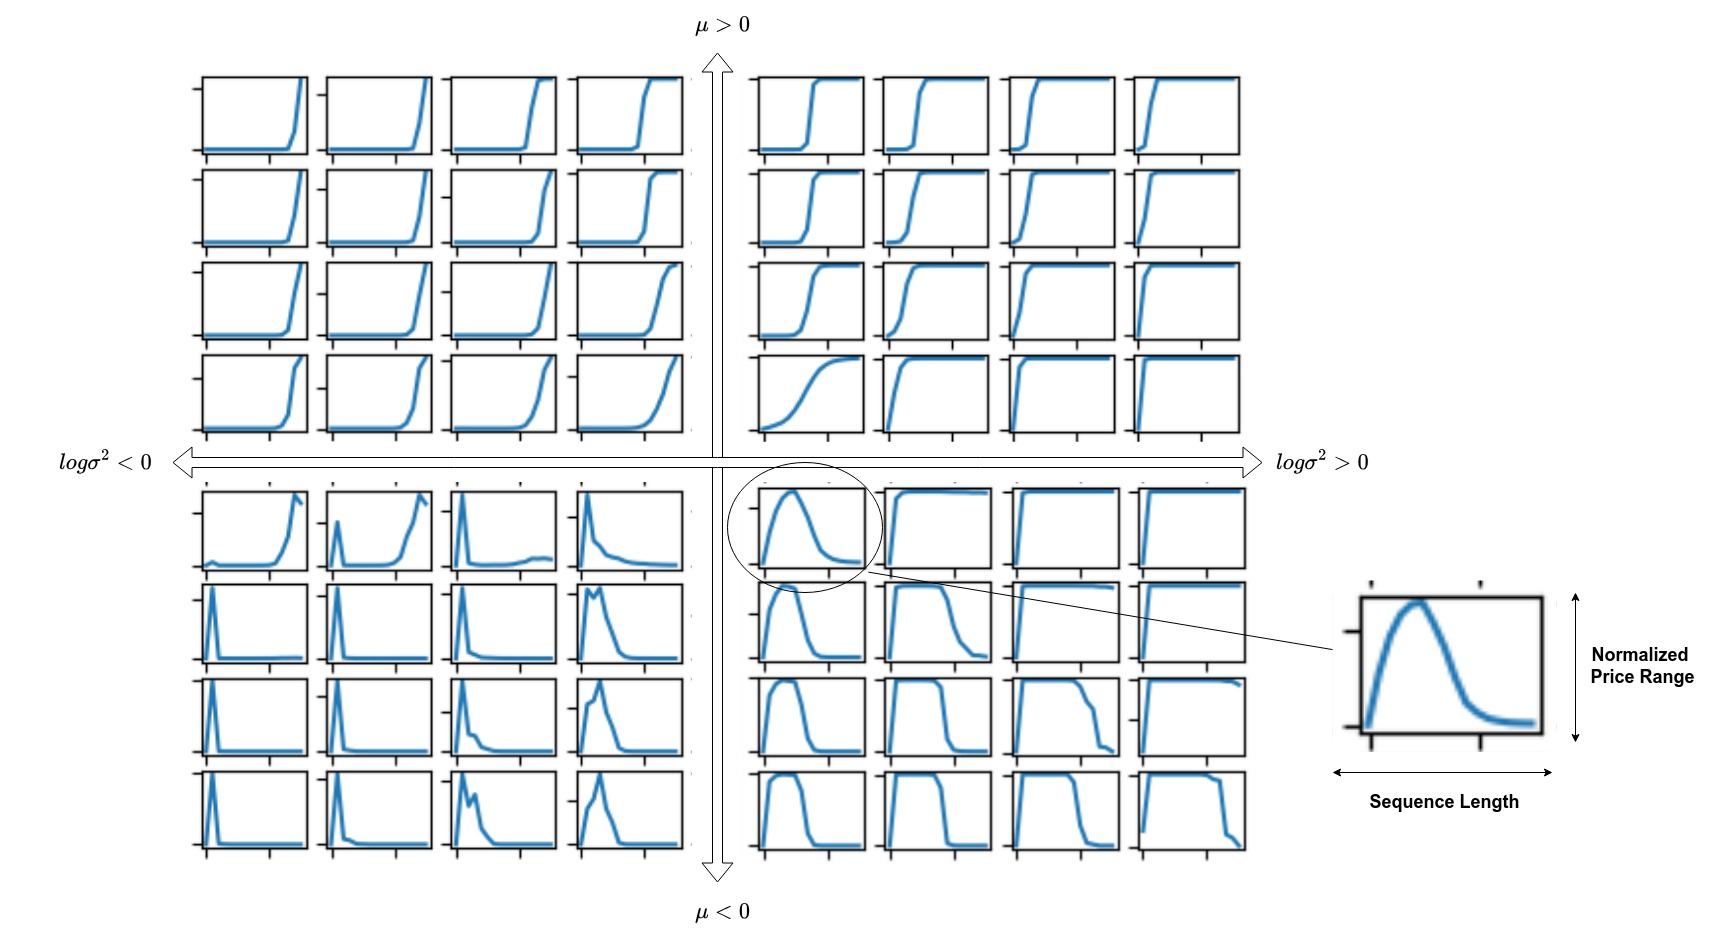
\includegraphics[scale=0.25]{./LatentSpace.jpg}
	\caption{Illustration of the latent space learned by VAE with classifier over model performance series}
	\label{fig:latent_full}
\end{figure}


\subsection{Ablation Study}

To assess the effectiveness of different components of the proposed method, we conduct an ablation study where we systematically analyze the impact of key elements such as the VAE for uncertainty measurement and the Actor-Critic neural network for stock portfolio proposal. By comparing the performance of the complete model with variations that exclude specific components, we aim to understand the contribution of each part to the overall coin switching strategy.

\subsubsection{Feature Extraction}
In the initial experiment in ablation study, our objective is to examine the influence of the VAE model on classification of price trend movement direction. For this aim, we utilize a multi-layer perceptron (MLP) network to categorize the direction of price movements based on the definition outlined in equation \eqref{eq:class1}. The outcomes of price trend prediction using various classifiers are compared in Table \ref{tbl:FE-pred}.

The baseline models considered in this study are as follows:
\begin{itemize}
	\item \textbf{MLP}. This model is a basic MLP classifier trained directly on the input series without any feature extraction.
	\item \textbf{VAE-Z}. Here, the VAE is trained, and only the embedding vector $Z$ is provided to the classifier as the extracted feature.
	\item \textbf{VAE-TR}. In this model, the VAE is trained, and the concatenated latent vectors $\hat{\mu}$ and $\hat{\sigma}$ are passed to the classifier as the extracted feature.
	\item \textbf{VAE-Y}. This model involves training the VAE, and only the VAE's embedded classifier output $\hat{Y} = \Phi(\hat{\mu}, \hat{\sigma})$ is used as the extracted feature.
	\item \textbf{VAE-FULL}. In this setup, the VAE is trained, and all encoder outputs containing $Z$, $\hat{\mu}$, and $\hat{\sigma}$ are concatenated and provided to the classifier as the extracted feature.
\end{itemize}

Table \ref{tbl:FE-pred} presents a comparison of the baseline models' accuracy in the classification task. The results indicate that model \textbf{VAE-Y} performs the best as a feature extractor. This observation supports our hypothesis that accurately predicting the likelihood of continuation of the current stock price trend can assist portfolio management models in determining optimal points for asset switching within the portfolio.

\begin{table}[h]
	\centering
	\caption{Comparison between baseline models accuracy in predicting the future price trend direction}
	\label{tbl:FE-pred}
	\begin{tabular}{c | c | c | c | c | c }
		Method & MLP & VAE-Z & VAE-TR & VAE-Y & VAE-FULL \\
		\hline
		\hline
		Train & 13.48 \%& 16.94 \%& 15.36 \%& \textbf{19.43} \%& 94.36 \%\\
		Test & 1.80 \%& 10.59 \%& 13.47 \%& \textbf{16.92} \%& 14.72 \%\\
	\end{tabular}
\end{table}

\subsubsection{Latent Space Dimensionality}
The following experiment aims to explore how the size of latent vectors $\hat{\mu}$ and $\hat{\sigma}$ influences the quality of extracted features. In this study, we varied the dimensions of the latent vectors and assessed the classifier's accuracy in predicting the next price movement direction.

The comparison of these models is presented in Table \ref{tbl:FE-dim}. The findings from this table suggest that enhancing the dimensionality of latent vectors leads to improved model performance. This improvement can be attributed to the larger latent vector size enabling the model to more effectively encapsulate the extracted information into a single vector. It is worth noting that as the dimensionality increases, more data is required for training, and therefore, performance gains may plateau after reaching a certain threshold with a fixed dataset size.


\begin{table}[h]
	\centering
	\caption{The impact of the latent vectors size on the accuracy of the price trend prediction}
	\label{tbl:FE-dim}
	\begin{tabular}{c | c | c | c | c | c }
		Method & 1 & 10 & 50 & 150 & 200 \\
		\hline
		\hline
		Train & 5.45& 6.02 & 18.51 & \textbf{19.43} \% & 18.46\\
		Test & 5.55& 4.16 & 13.37 & \textbf{16.92} \% & 15.24\\
	\end{tabular}
\end{table}

\subsubsection{Reward Function}
The reward function proposed for the coin-switching agent in equation \ref{eq:ri} is designed based on the distance between the selected coin by the agent and the best coin at each time step. This approach aims to give incentive to the agent to learn to switch to the best coin at every time step. Another commonly used reward function in this research domain is the total portfolio return at each time step. To evaluate the effectiveness of the proposed reward function, a comparison between these two models is presented in table \ref{tbl:rewards}. The table includes metrics such as total return on investment (\textbf{total-ROI}), maximum drawdown (\textbf{MDD}), and average return (\textbf{AR}) for each model. The results indicate that the model utilizing the proposed return function demonstrates superior performance compared to the traditional reward function commonly used in the field.


\begin{table}[h]
	\centering
	\caption{The impact of proposed reward function}
	\label{tbl:rewards}
	\begin{tabular}{c | c | c | c  }
		Method & total-ROI & MDD & AR \\
		\hline
		\hline
		Proposed Reward & \textbf{1850.44 \%}  & \textbf{-13.30 \%} & \textbf{0.0523}  \% \\
		Common Reward & 435.84 \%  & -25.48 \%  & 0.0151 \%\\
	\end{tabular}
\end{table}

%
%\subsubsection{Considering Risk-free Asset}
%One of the main underlying assumptions in our study was that mitigating minor losses would enhance portfolio management effectiveness. Consequently, we conducted an additional experiment to investigate how our model performs with and without the inclusion of a risk-free asset. Table \ref{tbl:rf1} presents a comparison of the model's performance under these conditions. The results indicate that the model performs better when the risk-free asset is included, particularly in terms of metrics such as maximum drawdown. This suggests that timely switching to the risk-free asset can help prevent losses in the investment process.
%
%\begin{table}[h]
%	\centering
%	\caption{The impact of risk-free asset presence on model's performance}
%	\label{tbl:rf1}
%	\begin{tabular}{c | c | c | c  }
%		Method & total-ROI & MDD & AR \\
%		\hline
%		\hline
%		with tether & \textbf{125 \%}  & \textbf{-19 \%} & \textbf{0.27}  \% \\
%		without tether & 28 \% & -34 \% & 0.11 \% \\
%	\end{tabular}
%\end{table}

%To demonstrate the efficiency of the proposed model in identifying and transitioning to the risk-free asset at opportune moments, we conducted an additional experiment. In this study, we defined periods where all coins exhibited a bearish price trend as bearish markets, with all other times classified as bullish. Subsequently, we evaluated the behavior of the coin-switching agent in terms of its ability to switch to the risk-free asset during bearish market conditions. The outcomes of this experiment are presented in Table \ref{tbl:rf2}. The true positive metric (TP) signifies the percentage of instances where the coin-switching agent correctly switched to the risk-free asset, while the false positive metric (FP) indicates the percentage of incorrect switches, and so forth. The results reveal that in the presence of a risk-free asset, the model effectively learns to transition to this asset when the majority of other coins are experiencing a bearish price trend. Our findings demonstrate that the coin-switching agent successfully switched to the risk-free asset in approximately 30\% of instances when all available coins were in a bearish trend.
%
%\begin{table}[h]
%	\centering
%	\caption{The confusion matrix of the proposed model indicating the power of the model in switching to the risk-free asset at proper times.}
%	\label{tbl:rf2}
%	\begin{tabular}{c | c | c }
%		Market & Positive & Negative \\
%		\hline
%		\hline
%		Positive & 0& 0 \\
%		Negative & 0& 0 \\
%	\end{tabular}
%\end{table}

%The experiment's results is summarized to compare various iterations of the proposed model. Table \ref{tbl:cmp1} presents the performance metrics of these models for comparison. The findings from the table indicate that the model utilizing \textbf{VAE-Y} as the feature extractor and incorporating the suggested reward function that accounts for the risk-free asset outperforms other versions of the model.

\subsection{Portfolio Proposals}
The primary objective of the proposed model is to identify optimal time points for transitioning between different coins in the market. While the model's primary focus is distinct from portfolio management in which models are supposed to propose a combination of instruments at each time-step, we conducted a performance evaluation by comparing it against both single asset trading strategies and portfolio management models to assess its effectiveness in identifying optimal transition points between coins.

\subsubsection{Baselines}
The baseline models that have been compared with the proposed model are outlined below:

\begin{itemize}
	\item \textbf{BaH(X)}\cite{li2014online}. This denotes the buy and hold strategy, where coin X is purchased at the beginning of the experiment and held until the end.
	%	\item \textbf{MLP-vanilla} \cite{taghian2022learning}.  This model, introduced by \cite{taghian2022learning}, involves a Deep Reinforcement Learning (DRL) model that learns candlestick patterns and establishes generalized trading rules for Bitcoin.
	\item \textbf{UCRP}\cite{li2014online}. Uniform Constant Rebalanced Portfolio strategy involves setting the portfolio proposal vector to a uniform vector $w^t=(\frac{1}{n}, \cdots, \frac{1}{n})$ at the start of each time step, where $n$ represents the number of available coins and $|w^t| = n$.	
	%	\item \textbf{FTW}. Following the winner strategy adjusts the portfolio proposal vector at each time step based on the historical performance of coins, with weights of winning coins revised according to their cumulative return $w^t = SoftMax(CR_t)$, where $CR_t$ is calculated as in equation \eqref{eq:ftw}.
	%	\begin{align}
	%		CR_t = \{R(X_i^{1:t})| \> &X_i^{1:t} = \{X_i^1, \cdots, X_i^t\} \> \land  \notag \\ 
	%		&R(X_i^{1:t}) = \frac{X_i^t}{X_i^1} \> \land \notag \\ 
	%		&i \in \{1, \cdots, n\}\}
	%		\label{eq:ftw}
	%	\end{align}
	%
	%	\item \textbf{FTL}. Following the loser strategy refines the portfolio proposal vector at the beginning of each time step by adjusting the weights of losing coins based on the inverse of their historical performance $w^t = SoftMax(CR_t^{-1})$, using $CR_t^{-1}$ computed as shown in equation \eqref{eq:ftl}.
	%	\begin{align}
	%	CR_t^{-1} = \{R(X_i^{1:t})^{-1} | &X_i^{1:t} = \{X_i^1, \cdots, X_i^t\} \> \land \notag\\ 
	%	&R(X_i^{1:t})^{-1} = \frac{1}{1 + log(\frac{X_i^t}{X_i^1})} \> \land \notag \\  
	%	&i \in \{1, \cdots, n\} \}
	%	\label{eq:ftl}
	%	\end{align}
\end{itemize}

\subsubsection{Deep Learning Models}
The state-of-the-art models that have been compared with the proposed model are outlined below:

\begin{itemize}
	\item \textbf{LSTM-GARCH}\cite{garcia2024lstm}. This approach employs a GARCH model to estimate the variance of each price series. The resulting variance estimates are then input into an LSTM network to generate portfolio vectors at each timestep.
	
	\item \textbf{Transformer}\cite{kumar2024transformer}. This model utilizes a Transformer network for price prediction, integrated with a DQN framework for decision-making.
	
\end{itemize}

For all the models discussed above, we implemented the proposed architectures as described in the original papers and conducted evaluations using our dataset to ensure consistency and reproducibility of the results.


\subsubsection{Comparison results}

Table \ref{tbl:cmp} presents the comparison of the performance of the proposed model against the baseline models in terms of total return on investment (RoI), maximum drawdown, and average return. In this table, the term $CoinSwitching^*$ represents the proposed model with the proposed reward function, which is considered the most effective version of the proposed model.

The results presented in the table highlight the significant outperformance of the proposed CoinSwitching model compared to both baseline strategies and deep learning models. CoinSwitching achieves a remarkable total-ROI of 1850.44\%, surpassing all other approaches by a wide margin, while maintaining the lowest Maximum Drawdown (MDD) of -13.30\%, indicating exceptional risk management and stability. The model's Annualized Return (AR) of 0.0523\% further underscores its superior capability in generating consistent and substantial profits. While baseline strategies such as BaH(XRP/BTC) and UCRP show occasional success, they fall short in overall performance and risk mitigation. Similarly, deep learning models, including LSTM-GARCH and Transformer, struggle with negative ROI and higher MDD, highlighting their limitations in adapting to the dynamic cryptocurrency environment.

In terms of Accuracy and Hit Rate, CoinSwitching demonstrates a well-balanced and robust performance. Although its Accuracy of 16.91\% is slightly lower than BaH(BNB/BTC) and Transformer, the high Hit Rate of 48.40\% indicates that it consistently selects coins with positive returns in the next time frame. This implies that CoinSwitching not only identifies profitable opportunities but also mitigates risks better than competing models. The impressive combination of high ROI, controlled MDD, and consistent Hit Rate validates the effectiveness of integrating transformer-based feature extraction with an Actor-Critic framework, showcasing its potential as a cutting-edge solution for dynamic portfolio management in volatile markets.

\begin{table}[h]
	\centering
	\caption{Comparison of the performance of the proposed model versus portfolio management, and single asset trading strategies.}
	\label{tbl:cmp}
	\begin{tabular}{l| c | c | c | c | c | c  }
		Model & total-ROI & MDD & AR & Accuracy & Hit Rate\\
		\hline
		\hline
		BaH(ETH/BTC) & -22.83 \%  & -44.03 \% & -0.0035 \% & 12.58 \% & 40.06 \% \\
		BaH(BTC/USDT) & 54.83 \%  & -30.53 \% &  0.0088 \% & 10.25 \% & 47.75 \% \\
		BaH(BNB/BTC) & -23.95 \%  & -38.45 \% &  -0.0035 \% & \textbf{17.99} \% & \textbf{50.92} \% \\
		BaH(XRP/BTC) & 201.69 \%  & -39.96 \% & 0.0224 \% & 14.17 \% & 41.07 \% \\
		BaH(LTC/BTC) & -7.34 \%  & -41.03 \% &  0.0011 \% & 12.89 \% & 41.64 \% \\
		BaH(ADA/BTC) & 24.07 \%  & -39.85 \% &  0.0067 \% & 6.70 \% & 45.47 \% \\
		BaH(DASH/BTC) & -15.98 \%  & -43.99 \% &  -0.0001 \% & 12.14 \% & 43.28 \% \\
		BaH(EOS/BTC) & -31.62 \%  & -59.88 \% & -0.0030 \% & 13.26 \% & 42.37 \% \\
		%										& MLP-vanilla \cite{taghian2022learning} & 248506 \%  & -82 \% & 1.87  \% \\
		UCRP & 17.76 \%  & -26.41 \% & 0.0036 \% & 12.58 \% & 40.06 \% \\
		\hline
		\hline
		LSTM-GARCH & -16.46 \%  & -52.79 \% & -0.0005 \% & 14.60 \% & 45.53 \% \\
		Transformer &  -32.29 \%  & -43.69 \% &  -0.0039 \% & 15.67 \% & 46.33 \% \\
		\hline
		\hline
		$CoinSwitching$ &  \textbf{1850.44} \%  & \textbf{-13.30} \%  & \textbf{0.0523} \% & 16.91 \% & 48.40 \% \\
	\end{tabular}
\end{table}

Furthermore, the diagram in Figure \ref{fig:versions} illustrates the evolution of portfolio values for various strategies over time. It is evident from the graph that the suggested approach outperforms other strategies by mitigating minor losses. While different segments of the proposed strategy's portfolio value curve resemble those of other strategies, the key distinction lies in its ability to avert losses by switching between selected coins, thereby enhancing overall portfolio performance significantly.

\begin{figure}[h]
	\centering
	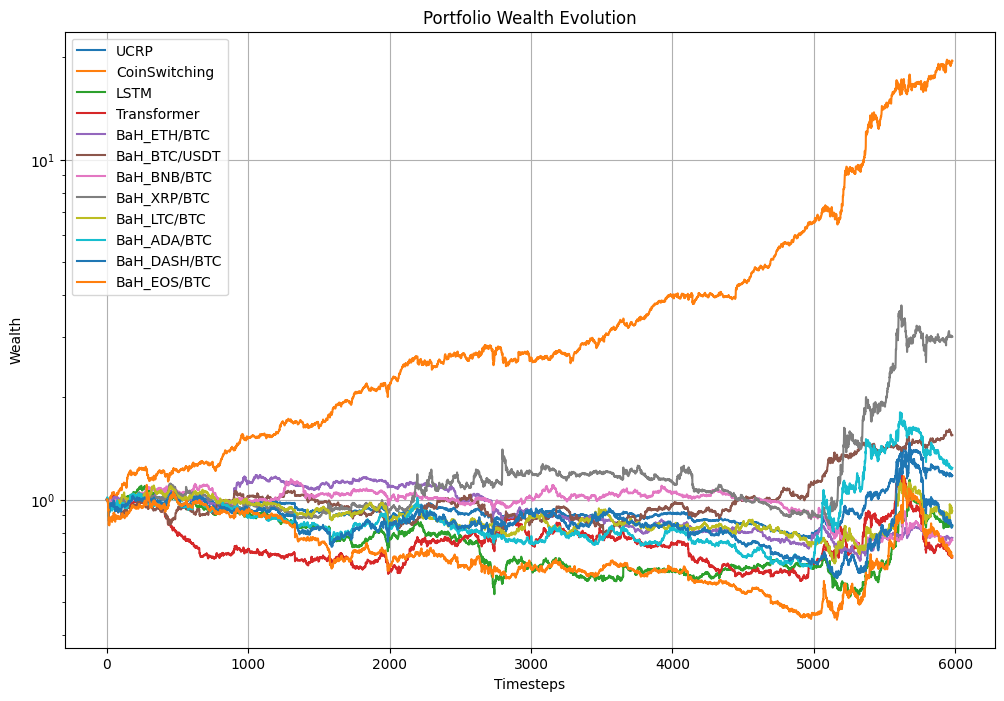
\includegraphics[scale=0.6]{./ms1.png}
	\caption{Comparison of the proposed model with single asset strategies.}
	\label{fig:versions}
\end{figure}

Moreover, Figure \ref{fig:changes1} depicts the behaviors of different strategies over the investment period. The portfolio weight visualization underscores the innovation of the CoinSwitching strategy, where the entire investment is allocated dynamically to a single coin at the beginning of each investment period. This chart clearly differentiates the CoinSwitching model from traditional strategies such as UCRP and baseline "Buy-and-Hold" (BaH) approaches. Unlike these methods, which either distribute weights equally or fix them to a specific coin, CoinSwitching actively reallocates 100\% of the portfolio to the coin predicted to show the most favorable trend. This decisive and focused approach enables the model to capitalize on high-probability opportunities, minimizing exposure to underperforming assets.

The chart further illustrates how this single-coin allocation strategy functions effectively as a dynamic diversification mechanism over time. By successively switching to the most promising coin based on predicted trend shifts, CoinSwitching emulates the cumulative benefits of diversification while avoiding dilution of returns across less favorable coins. This behavior mirrors the concept of concurrent task execution in CPU processing, where tasks are processed in rapid succession to achieve efficiencies akin to parallel computation. The ability to adapt to market conditions dynamically, coupled with disentangled trend and variance predictions, ensures that the portfolio remains agile and optimized, maximizing returns while controlling risk in volatile cryptocurrency markets.


\begin{figure}[H]
	\centering
	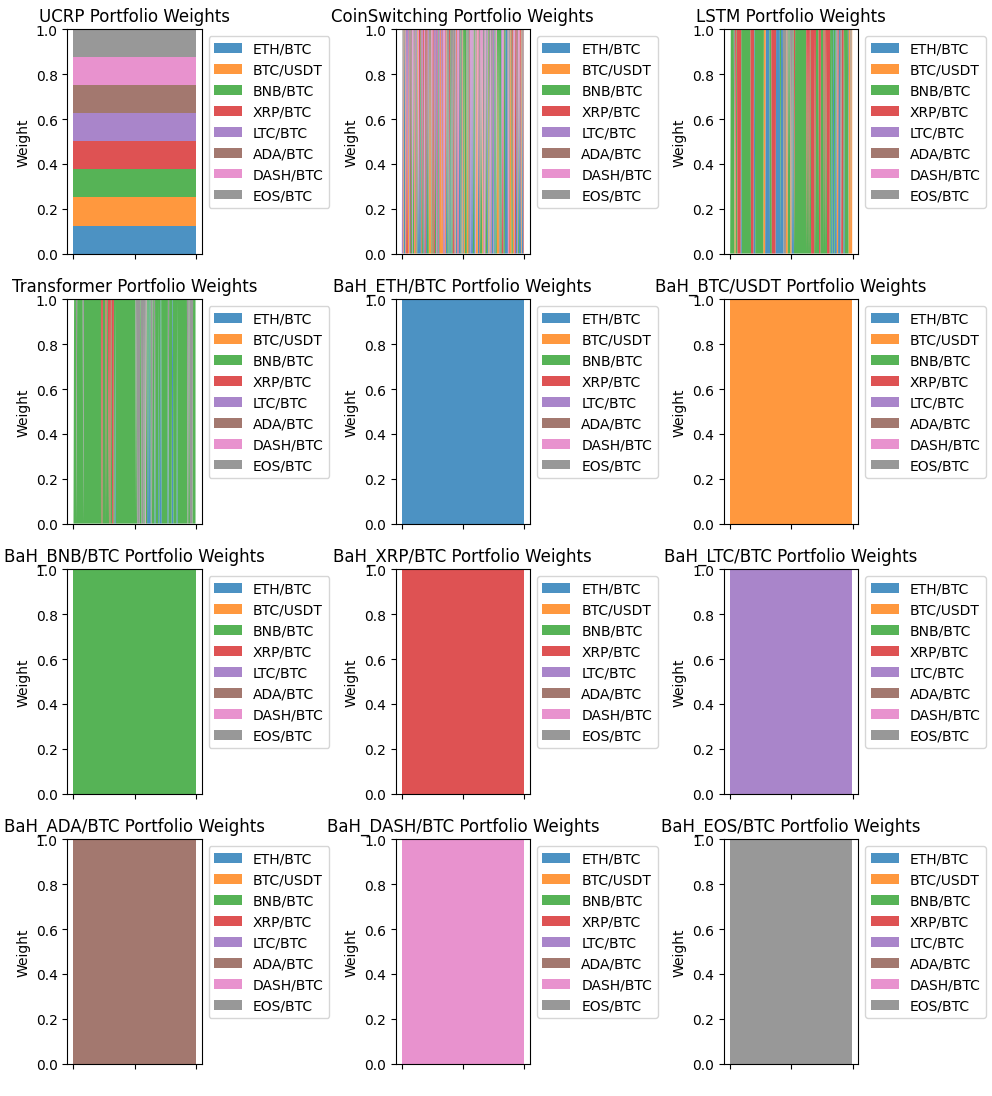
\includegraphics[scale=0.45]{./changes1.png}
	\caption{Model selection during investment timesteps}
	\label{fig:changes1}
\end{figure}





\section{Conclusion}


In conclusion, the proposed model for stock portfolio management in the cryptocurrencies market demonstrates several key advantages and some limitations that are important to consider:

\subsection{Advantages}

\begin{enumerate}
	\item Effective uncertainty estimation: The integration of a Variational Autoencoder (VAE) enables our model to accurately quantify uncertainty in stock price predictions, providing valuable insights for risk management and decision-making.
	
	\item Dynamic portfolio optimization: The Actor-Critic neural network architecture allows for adaptive and dynamic portfolio rebalancing based on changing market conditions, leading to improved performance and resilience against volatility.
	
	%	\item Robust Performance: Through extensive experimentation and comparison with state-of-the-art models, our method consistently achieves competitive results in terms of return on investment, Sharpe ratio, and maximum drawdown, showcasing its effectiveness in generating optimal stock portfolios.
	
	\item Real-world applicability: Leveraging a comprehensive dataset of historical cryptocurrency prices, our model operates under realistic market conditions, enhancing its practical relevance and applicability for financial institutions and investors.
	
\end{enumerate}


\subsection{Weaknesses}

\begin{enumerate}
	%	\item Complexity: The complexity of the proposed model, particularly the integration of multiple neural network components and hyperparameters, may pose challenges in implementation and interpretation for users without a deep understanding of machine learning techniques.
	
	\item Data dependency: The performance of our model heavily relies on the quality and availability of historical asset price data during the training phase, which may limit its effectiveness in scenarios where data is scarce or unreliable.
	
	%	\item Training Time: Training neural networks for portfolio optimization can be computationally intensive and time-consuming, especially when dealing with large datasets and complex architectures, potentially hindering real-time decision-making processes.
	
\end{enumerate}


Overall, the benefits of the proposed model outweigh its limitations, as it offers a data-driven approach to assess uncertainty of price trends in stock portfolio management in the volatile cryptocurrencies market. By addressing uncertainties and optimizing portfolios dynamically,giggg our method provides a valuable tool for investors seeking to navigate the complexities of cryptocurrency trading with enhanced confidence and efficiency. Further research and refinement of the model could help mitigate its limitations and unlock even greater potential for AI-driven financial strategies in the future.








%\bibliographystyle{elsarticle-num-names} 
\bibliography{references}


\end{document}
